%\documentclass[a4paper,twocolumn]{article} % Document type

\documentclass[a4paper,12pt,oneside,onecolumn]{article} % Document type

\usepackage[left=1.0in, right=1.0in, top=1.0in, bottom=1.0in]{geometry}

\ifx\pdfoutput\undefined
    %Use old Latex if PDFLatex does not work
   \usepackage[dvips]{graphicx}% To get graphics working
   \DeclareGraphicsExtensions{.eps} % Encapsulated PostScript
 \else
    %Use PDFLatex
   \usepackage[pdftex]{graphicx}% To get graphics working
   \DeclareGraphicsExtensions{.pdf,.jpg,.png,.mps} % Portable Document Format, Joint Photographic Experts Group, Portable Network Graphics, MetaPost
   \pdfcompresslevel=9
\fi

\usepackage{amsmath,amssymb}   % Contains mathematical symbols
\usepackage[ansinew]{inputenc} % Input encoding, identical to Windows 1252
\usepackage[english]{babel}    % Language
\usepackage[square,numbers]{natbib}     %Nice numbered citations
\bibliographystyle{plainnat}            %Sorted bibliography



\begin{document}               % Begins the document

\title{Homework 1 in EL2450 Hybrid and Embedded Control Systems}
\author{
  Ahmed Alhaidari \\ 901009-3335 \\ aalh@kth.se 
  \and 
  Yue Jiao \\ 911024-7799 \\ yj@kth.se
  }
%\date{2010-10-10}             % If you want to set the date yourself.

\maketitle                     % Generates the title



\section*{Task 1}
The value of $\theta_{c_i}$ can be found from geometry as the following: 
\begin{equation}
    \theta_{c_1} = q_1 , \qquad \theta_{c_1} = q_1 + q_2
\end{equation}

Additional geometry shall give the position of the mass of the arm links: 
\begin{equation}
    \begin{aligned}
        p_{c_1} & = [l_{c_1}  \cos{\theta_{c_1}}, \quad l_{c_1}  \sin{\theta_{c_1}}]^T \\ 
                & = [l_{c_1}  \cos{q_1}, \quad l_{c_1}  \sin{q_1}]^T \\
        p_{c_2} & = [l_1  \cos{\theta_{c_1}} + l_{c_2}   \cos{\theta_{c_2}}, \quad    l_1  \sin{\theta_{c_1}} +  l_{c_2}   \sin{\theta_{c_2}}]^T \\ 
                & = [l_1  \cos{q_1} + l_{c_2}   \cos{(q_1+q_2)}, \quad l_1  \sin{q_1} +  l_{c_2}   \sin{(q_1+q_2)}]^T 
    \end{aligned}
\end{equation}

So the total expression can be written as:
\begin{equation}
    \begin{bmatrix}
    p_{c_1}^T \\ \theta_{c_1}
    \end{bmatrix} = 
    \begin{bmatrix}
    l_{c_1}  \cos{q_1} \\ l_{c_1}  \sin{q_1} \\ q_1 \\
    \end{bmatrix}
\end{equation}
and
\begin{equation}
    \begin{bmatrix}
    p_{c_2}^T \\ \theta_{c_2}
    \end{bmatrix} = 
    \begin{bmatrix}
    l_1  \cos{q_1} + l_{c_2}   \cos{(q_1+q_2)} \\ l_1  \sin{q_1} +  l_{c_2}   \sin{(q_1+q_2)} \\ q_1 + q_2 \\
    \end{bmatrix}
\end{equation}


\section*{Task 2}
By the definition, $v_{c_i} = [\dot{p}^T_{c_i}, \omega_{c_i}]^T =[\dot{p}^T_{c_i}, \dot{\theta}_{c_i}]^T$ which can be calculated by mathematical analysis: 
\begin{equation}
    \begin{aligned}
        \dot{\theta}_{c_1} & = \dot{q_1} \\ \dot{\theta}_{c_2} & = \dot{q_1} + \dot{q_2} \\
        \dot{p}_{c_1} & = [-\dot{q}_1 l_{c_1}  \sin{q_1}, \quad \dot{q}_1 l_{c_1}  \cos{q_1}]^T \\
        \dot{p}_{c_2} & = [-\dot{q}_1 l_1  \sin{q_1} - (\dot{q}_1+\dot{q}_2) l_{c_2}   \sin{(q_1+q_2)}, \quad \dot{q}_1 l_1 \cos{q_1} +  (\dot{q}_1+\dot{q}_2) l_{c_1}  \cos{(q_1+q_2)}]^T 
    \end{aligned}
\end{equation}

This can be written in the following matrix form $v_{c_i} = J_i(q) \dot{q}$ where $J_i$ is the Jacobians matrix. 

\begin{equation}
    \begin{bmatrix}
    v_{c_1}
    \end{bmatrix} = 
    \begin{bmatrix} 
    -l_{c_1}  \sin{q_1} & 0  \\ \quad l_{c_1}  \cos{q_1} & 0 \\ 1 & 0 \\
    \end{bmatrix}
    \begin{bmatrix}
    \dot{q_1} \\ \dot{q_2} \\
    \end{bmatrix} 
\end{equation}
and
\begin{equation}
    \begin{bmatrix}
    v_{c_2}
    \end{bmatrix} = 
    \begin{bmatrix} 
    -l_1  \sin{q_1} - l_{c_2}  \sin{(q_1 + q_2)}  & -l_{c_2}  \sin{(q_1 + q_2)}  \\ \quad l_1 \cos{q_1}  + l_{c_2}  \cos{(q_1 + q_2)}  & l_{c_2}  \cos{(q_1 + q_2)} \\ 1 & 1 \\
    \end{bmatrix}
    \begin{bmatrix}
    \dot{q_1} \\ \dot{q_2} \\
    \end{bmatrix} 
\end{equation}

\section*{Task 3}
According to the mechanical engineering, the kinetic energy and potential energy can be expressed in the following way: $K_i = \frac{1}{2} m_i v_i^2 + \frac{1}{2} I_i \omega_i^2$, $P_i = m_i g p_{c_i, y}$. So the Lagrangian function is then $L_i = K_i - P_i$. The Lagrangian function with expressions from above plugged in shall have the form like the following:
\begin{equation}
\begin{aligned}
L_1 & = \frac{1}{2} m_1 l_{c_1}^2 \dot{q}_1^2 + \frac{1}{2} I_1 \dot{q}_1^2 - m_1 g l_{c_1} \sin{q_1} \qquad \Rightarrow \\
\frac{\partial}{\partial t}(\frac{\partial L_1}{\partial \dot{q}_1}) - \frac{\partial L_1}{\partial q_1} & = m_1 l_{c_1}^2 \ddot{q}_1 + I_1 \ddot{q}_1 + m_1 g l_{c_1} \cos{q_1} \\
\frac{\partial}{\partial t}(\frac{\partial L_1}{\partial \dot{q}_2}) - \frac{\partial L_1}{\partial q_2} & = 0
\end{aligned}
\end{equation}
and
\begin{equation}
\begin{aligned}
L_2 = & \frac{1}{2} m_2 l_1^2 \dot{q}_1^2 + \frac{1}{2} m_2 l_{c_2}^2 (\dot{q}_1 + \dot{q}_2)^2 + m_2 l_1 l_{c_2} \dot{q}_1 (\dot{q}_1 + \dot{q}_2) \cos{q_2} \\ 
& + \frac{1}{2} I_2 (\dot{q}_1 + \dot{q}_2)^2  - m_2 g (l_1 \sin{q_1} + l_{c_2}\sin{(q_1+q_2)}) \qquad \Rightarrow \\
\frac{\partial}{\partial t}(\frac{\partial L_1}{\partial \dot{q}_1}) - \frac{\partial L_1}{\partial q_1} = & m_2 l_1^2 \ddot{q}_1 + m_2 l_{c_2}^2 (\ddot{q}_1+\ddot{q}_2) + m_2 l_1 l_{c_2} (2\ddot{q}_1 + \ddot{q}_2) \cos{q_2} \\
& - m_2 l_1 l_{c_2} \dot{q}_2 (2\dot{q}_1 + \dot{q}_2) \sin{q_2} + I_2 (\ddot{q}_1 + \ddot{q}_2) \\
& + m_2 g l_1 \cos{q_1} + m_2 g l_{c_2} \cos{(q_1 + q_2)} \\
\frac{\partial}{\partial t}(\frac{\partial L_1}{\partial \dot{q}_2}) - \frac{\partial L_1}{\partial q_2} = & m_2 l_{c_2}^2 (\ddot{q}_1 + \ddot{q}_2)  + m_2 l_1 l_{c_2} \ddot{q}_1 \cos{q_2} \\
& + m_2 l_1 l_{c_2}\dot{q}_1^2 \sin{q_2} + I_2 (\ddot{q}_1 + \ddot{q}_2) + m_2 g l_{c_2} \cos{q_1 + q_2}
\end{aligned}
\end{equation}

Then the Lagrangian formulation can be calculated as $L = L_1 + L_2$ and
\begin{equation}
\frac{\partial}{\partial t}(\frac{\partial L}{\partial \dot{q}_i}) - \frac{\partial L}{\partial q_i} = \frac{\partial}{\partial t}(\frac{\partial L_1}{\partial \dot{q}_i}) - \frac{\partial L_1}{\partial q_i} + \frac{\partial}{\partial t}(\frac{\partial L_2}{\partial \dot{q}_i}) - \frac{\partial L_2}{\partial q_i}
\end{equation}

This expression can be rewritten in matrix form $B(q)\ddot{q} + N(q, \dot{q})\dot{q}+P_g(q) = \tau$. Here $B(q)$ can be calculated easily by pick elements containts $\ddot{q}_i$. The elements in matrix $N$ can be calculated in the following way: 
Let $B=[b_{ij}]$. 
\begin{equation}
    n_{ij} = \sum_{k=1}^2 n_{ijk} \dot{q}_k 
\end{equation}
where
\begin{equation}
    n_{ijk} = \frac{1}{2} (\frac{\partial b_{ij}}{\partial q_k} + \frac{\partial b_{ik}}{\partial q_j} - \frac{\partial b_{jk}}{\partial q_i})
\end{equation}

In total the Lagrangian formulation can be written in the following way:
\begin{equation}
\begin{aligned}
    \begin{bmatrix}
    m_1 l_{c_1}^2 + I_1 + m_2 l_1^2 + m_2 l_{c_2}^2 + I_2 + 2 m_2 l_1 l_{c_2} \cos{q_2} &  m_2 l_{c_2}^2 + I_2 + m_2 l_{c_1} l_{c_2} \cos{q_2} \\
    m_2 l_{c_2}^2  + I_2 + m_2 l_{c_1} l_{c_2} \cos{q_2} &  m_2 l_{c_2}^2 + I_2 \\
    \end{bmatrix}
    \begin{bmatrix}
    \ddot{q}_1 \\ \ddot{q}_2 \\
    \end{bmatrix} & + \\
    \begin{bmatrix}
    - m_2 l_{c_1} l_{c_2} \dot{q}_2 \sin{q_2}  & - m_2 l_{c_1} l_{c_2} (\dot{q}_1+\dot{q}_2) \sin{q_2}  \\
      m_2 l_{c_1} l_{c_2}\dot{q}_1 \sin{q_2}  & 0
    \end{bmatrix}
    \begin{bmatrix}
    \dot{q}_1 \\ \dot{q}_2 \\
    \end{bmatrix} & + \\
    \begin{bmatrix}
    - 2 m g l_{c_1} \sin{q_1} - m g l_{c_2}   \sin{(q_1+q_2)} \\  - m g l_{c_2} \cos{(q_1 + q_2)} \\
    \end{bmatrix} & = \tau
\end{aligned}
\end{equation}

With these matrices it is easy to check that the following condition fulfills: 
\begin{equation} \label{eq:B-2N}
    \dot{B}-2N = -(\dot{B}-2N)^T = 
    \begin{bmatrix}
    0 & (2\dot{q}_1 + \dot{q}_2) m l_{c_1} l_{c_2} \sin{q_2} \\
    -(2\dot{q}_1 + \dot{q}_2) m l_{c_1} l_{c_2} \sin{q_2} & 0 \\
    \end{bmatrix}
\end{equation}



\section*{Task 4}
Here the controller is set to be the following form: 
\begin{equation}
    \tau = P_g - K_v \dot{q} - K_p e
\end{equation}

Insert it into the dynamic model: 
\begin{equation}\label{eq:cont}
\begin{aligned}
    B \ddot{q} + N \dot{q} + P_g = P_g - K_v \dot{q} - K_p e  \Rightarrow
    K_v \dot{q} + K_p e + B \ddot{q} + N \dot{q} = 0 
\end{aligned}
\end{equation}

So,

\begin{equation} \label{eq:Bq}
\begin{aligned}
     B \ddot{q}= -K_v \dot{q} - K_p e - N \dot{q}
\end{aligned}
\end{equation}

Let the Lyapunov equation for this system be $V = \frac{1}{2} e^T K_p e + \frac{1}{2} \dot{q}^T B(q) \dot{q}$. 

Now, taking the derivative of $V$ with respect to time gives the following equation: 
\begin{equation} \label{eq:dV0}
\begin{aligned}
\dot{V} = e^T K_p \dot{e} + \frac{1}{2} \dot{q}^T \dot {B(q)} \dot{q} + \frac{1}{2} \ddot{q}^T B(q) \dot{q} + \frac{1}{2} \dot{q}^T B(q) \ddot{q}
\end{aligned}
\end{equation} 

Since the off-diagonal element of the positive definite inertia matrix $B$ are the equal, the last two terms of equation [\ref{eq:dV0}] can be combined as follows: 

\begin{equation} \label{eq:dV}
\begin{aligned}
\dot{V}= e^T K_p \dot{e} + \frac{1}{2} \dot{q}^T \dot {B(q)} \dot{q} + \dot{q}^T B(q) \ddot{q}
\end{aligned}
\end{equation} 

Knowing that $\dot{e}=\dot{q}$ then substituting equation [\ref{eq:Bq}] into [\ref{eq:dV}]: 

\begin{equation} \label{eq:dV2}
\begin{aligned}
\dot{V} = e^T K_p \dot{q} - \dot{q}^T K_p e + \frac{1}{2} \dot{q}^T (\dot{B}-2N) \dot{q} - \dot{q}^T K_v \dot{q}
\end{aligned}
\end{equation}

Only the last term of equation [\ref{eq:dV2}] is not zero. The $\dot{B}-2N$ is skew-symmetric, see equation [\ref{eq:B-2N}], and the $K_p$ is symmetric, and therefore they are zeros. So,

\begin{equation} \label{eq:dV3}
\begin{aligned}
\dot{V} = - \dot{q}^T K_v \dot{q}
\end{aligned}
\end{equation}

From Lasalle's invariance principle, the one can deduce that the proposed controller achieves asymptotic stability since  $\dot{V} \leq 0$ and it is only equal to $0$ at $\dot{q}=0$ which is where $e=0$, see equation {\ref{eq:cont}}.


\section*{Task 5}
The system and controller above is implemented in Simulink. Several values of $K_v$ and $K_p$ are tested. Higher values of $K_v$ and $K_p$ give a faster responding system and less oscillating system, but the rise time increases slightly with the increases in the values of $K_v$ and $K_p$.

The desired value chosen is $q_{1,des} = \pi/2$ and $q_{2,des} = 0$. The step response for $q_1$ and $q_2$ at $K_p,K_v=3$ is shown in figure \ref{fig:0}

\begin{figure}[ht]
    \centering
    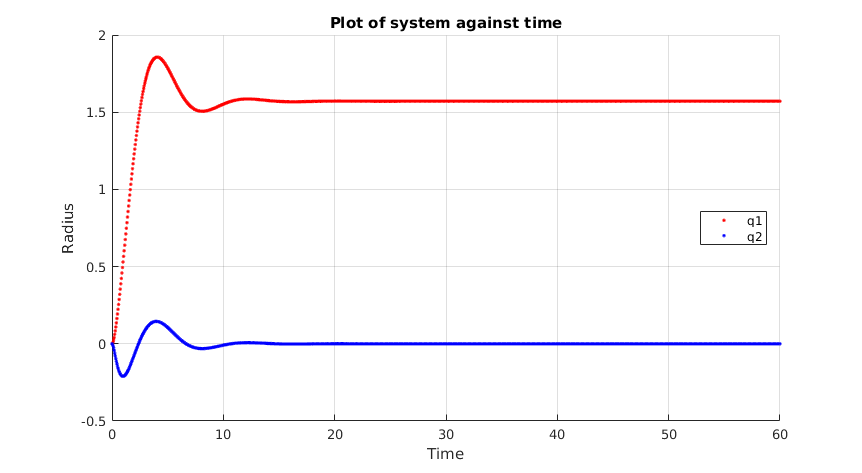
\includegraphics[scale=0.4]{cont_3_3.png}
    \caption{Testing the controller for $K_v=3$ and $K_p=3$}
    \label{fig:0}
\end{figure} 

%% Here come the plots cont_x_y where x is Kv and y is Kp

\section*{Task 6}
Now two zero-order-hold blocks are added to the simulation between the controller and the measurement of $q$ and $\dot{q}$. For comparison and analysis, different values of sampling time are simulated with $K_v = K_p = 3$ as a reference. 

The simulation results are showed in figure \ref{fig:1} and \ref{fig:2} for sampling time of 0.20 and 0.3 respectively.

\begin{figure}[ht]
    \centering
    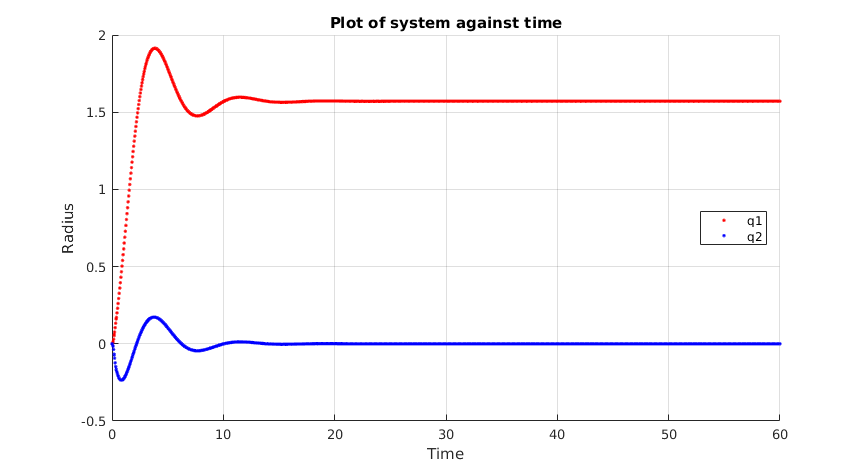
\includegraphics[scale=0.4]{zoh_20.png}
    \caption{Sampled controller test for $T=0.20$}
    \label{fig:1}
\end{figure} 

\begin{figure}[ht]
    \centering
    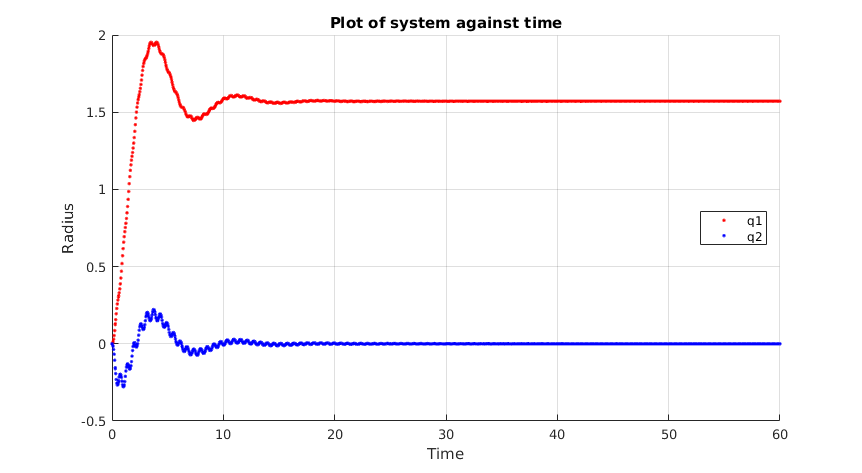
\includegraphics[scale=0.4]{zoh_30.png}
    \caption{Sampled controller test for $T=0.30$}
    \label{fig:2}
\end{figure} 

%% Here come the plots zoh_xx where xx is sampling time of both ZOH.

It can be seen that the system is not always stable for all values of sampling time. The system become unstable when the sampling time reach $0.40$. 

\section*{Task 7}
In this task, three additional quantizers are added. Two of them are between the controller and the zero-order-hold. The other one of them are between the controller and the input to the arm. 

To compare and then analys the results different values of the quantizer are tested under the same condition. The controller is set to $K_v = K_p =3$ and both of the zero-order-hold have the sampling time $0.30$. 

The simulation results are shown in figure \ref{fig:3} and \ref{fig:4}:

\begin{figure}[ht]
    \centering
    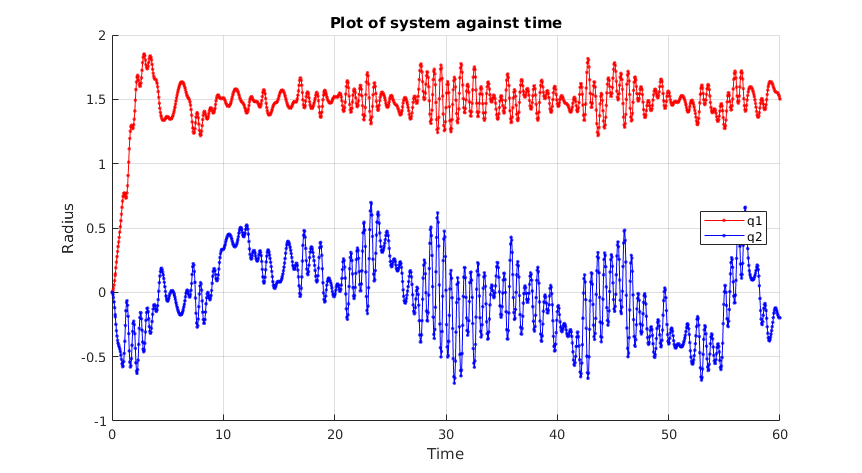
\includegraphics[scale=0.4]{quant_1_1.png}
    \caption{Sampled controller test with quantization module for 1 degree and 1Nm levels}
    \label{fig:3}
\end{figure} 

\begin{figure}[ht]
    \centering
    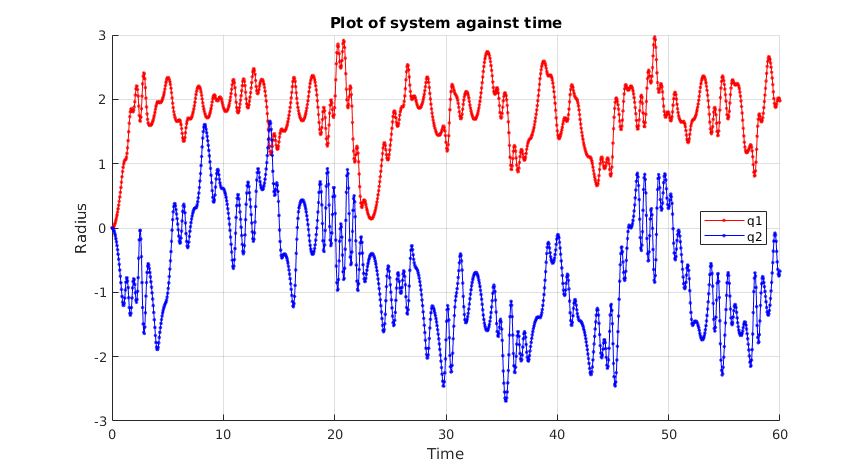
\includegraphics[scale=0.4]{quant_4_4.png}
    \caption{Sampled controller test with quantization module for 4 degree and 4Nm levels}
    \label{fig:4}
\end{figure}  


%% Here come the plots quant_xx_yy where xx is quant between ZOH and controller, yy is quant between controller and arm. 


\section*{Task 8}
Now the controller is changed to the following one: 
\begin{equation}
    \tau = B \dot{v}_{des} + N v_{des} + P_g - K_p e - K_v e_v
\end{equation}
Here
\begin{equation}
    v_{des} = \dot{q}_{des} - e \Rightarrow \dot{v}_{des} = \ddot{q}_{des} - \dot{e} =  \ddot{q}_{des} - (\dot{q} - \dot{q}_{des})
\end{equation}
and 
\begin{equation}
    e_v = \dot{q} - v_{des} \Rightarrow \dot{e_v} = \ddot{q} - \dot{v_{des}}
\end{equation}

Take the derivative of $V$ with respect to time gives the following equation:

\begin{equation}
    e_v = \dot{e}^T K_p \dot{e} + \frac{1}{2}\dot{e}^T K_p \dot{e}
\end{equation}

\section*{Task 9}
The system is simulated with the controller above. To make the simulation more interesting, the desired angles, angular velocity and angular acceleration are set to the following values:
\begin{equation}
    \begin{bmatrix}
    q_{1,des} \\ q_{2,des}
    \end{bmatrix} = 
    \begin{bmatrix}
    \frac{\pi}{2} \\ \frac{\pi}{4}\sin(0.5t)
    \end{bmatrix} , \quad
    \begin{bmatrix}
    \dot{q}_{1,des} \\ \dot{q}_{2,des}
    \end{bmatrix} = 
    \begin{bmatrix}
    0 \\ 0.5 \frac{\pi}{4} \cos{0.5t}
    \end{bmatrix} , \quad
    \begin{bmatrix}
    \ddot{q}_{1,des} \\ \ddot{q}_{2,des}
    \end{bmatrix} = 
    \begin{bmatrix}
    0 \\ -0.5^2 \frac{\pi}{4} \sin{0.5t}
    \end{bmatrix} 
\end{equation}

The simulation results are shown in \ref{fig:5} and \ref{fig:6}.

\begin{figure}[ht]
    \centering
    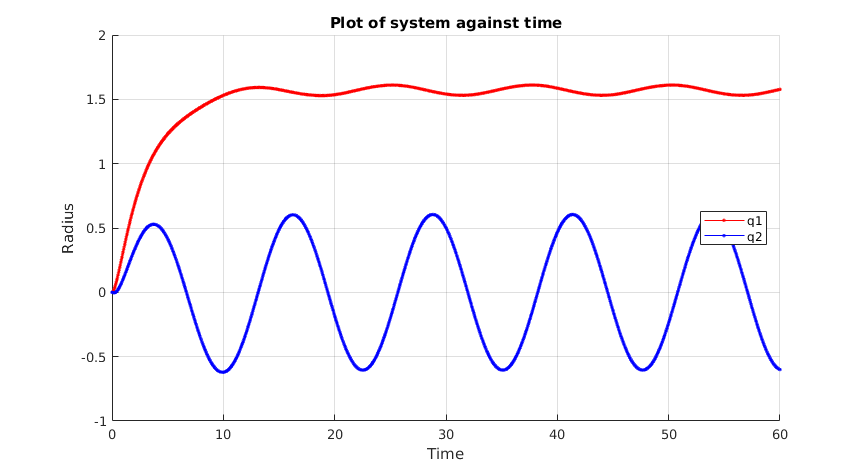
\includegraphics[scale=0.4]{cont2_3_3.png}
    \caption{Testing the controller for $K_v=3$ and $K_p=3$}
    \label{fig:5} 
\end{figure} 

\begin{figure}[ht]
    \centering
    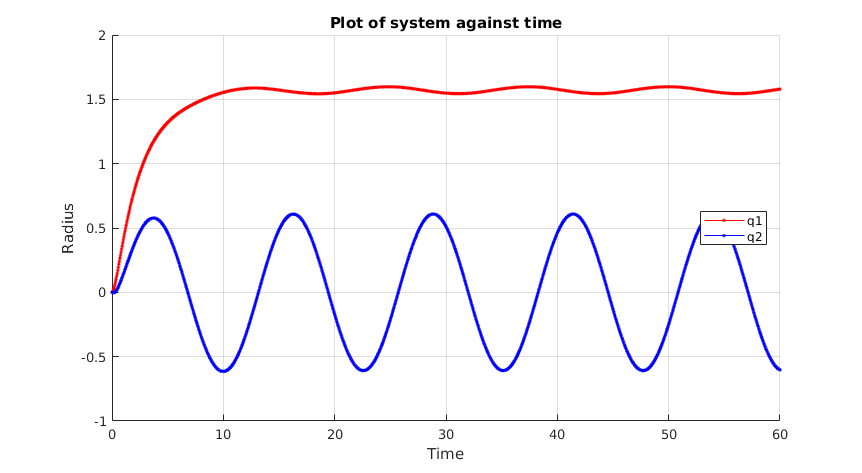
\includegraphics[scale=0.4]{cont2_5_5.png}
    \caption{Testing the controller for $K_v=5$ and $K_p=5$}
    \label{fig:6}
\end{figure} 


%% Here come the plots cont2_x_y

\section*{Task 10}
A similar test with zero-order-hold is done on this controller. As the task above, the parameters of the controller are set to $K_v = K_p = 3$. 
The simulation results are shown in figure \ref{fig:7}, \ref{fig:8} and \ref{fig:9}. 

\begin{figure}[ht]
    \centering
    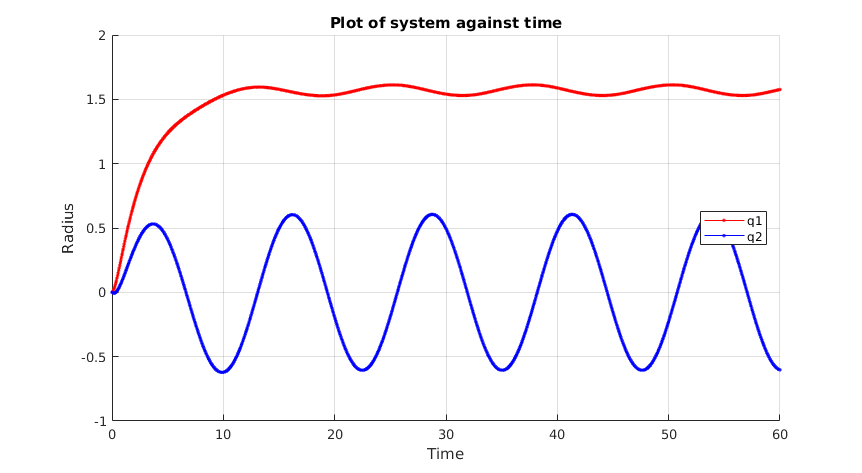
\includegraphics[scale=0.4]{zoh2_10.png}
    \caption{Sampled controller test for $T=0.10$}
    \label{fig:7}
\end{figure} 

\begin{figure}[ht]
    \centering
    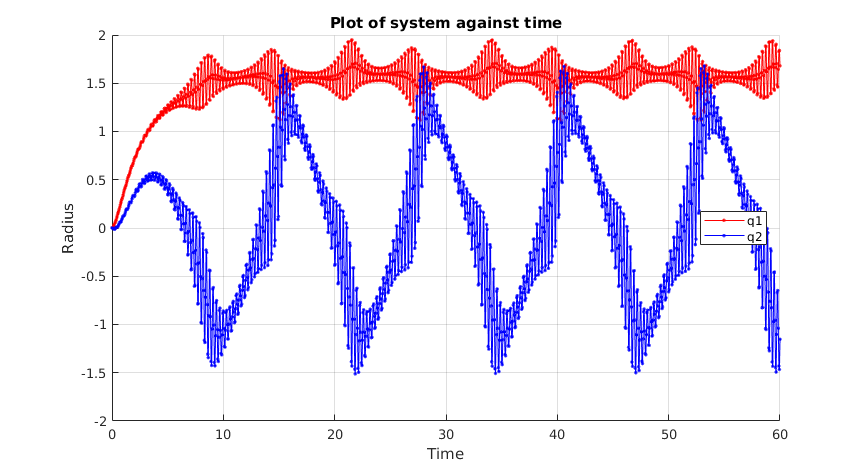
\includegraphics[scale=0.4]{zoh2_15.png}
    \caption{Sampled controller test for $T=0.15$}
    \label{fig:8}
\end{figure}  

\begin{figure}[ht]
    \centering
    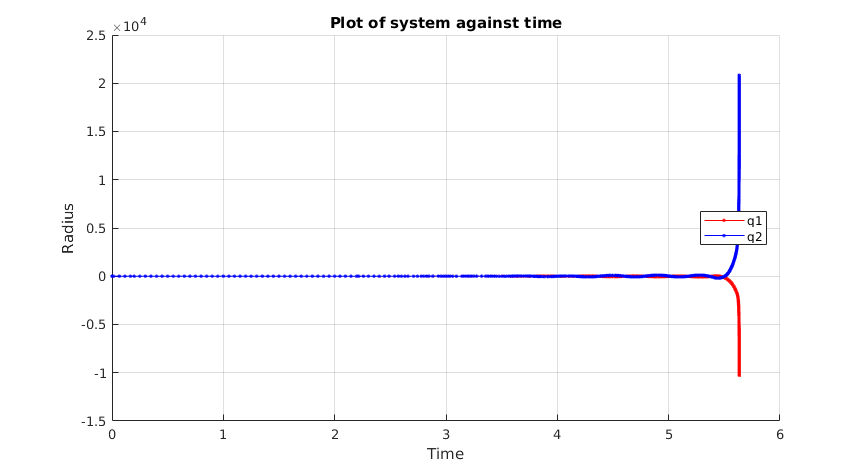
\includegraphics[scale=0.4]{zoh2_20.png}
    \caption{Sampled controller test for $T=0.20$}
    \label{fig:9}
\end{figure}  


%% Here come the plots zon2_xx

\section*{Task 11}
A similar test with quantizers and zero-order-hold is done on this controller. Since the sampling time cannot be as big as $0.30$, the sampling time for this test is set to $0.10$ and parameters of the controller are $K_v = K_p = 3$. The simulation results are shown in figure \ref{fig:10} and \ref{fig:11}

\begin{figure}[ht]
    \centering
    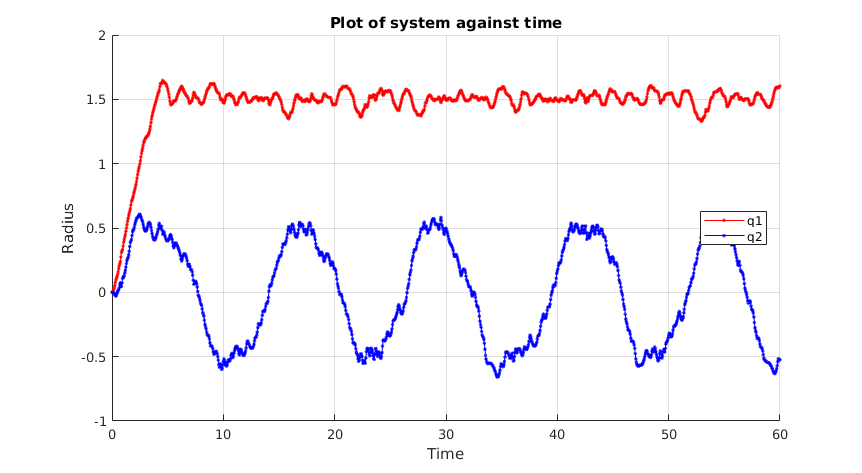
\includegraphics[scale=0.4]{quant2_1_1.png}
    \caption{Sampled controller test with quantization module for 1 degree and 1Nm levels}
    \label{fig:10}
\end{figure} 

\begin{figure}[ht]
    \centering
    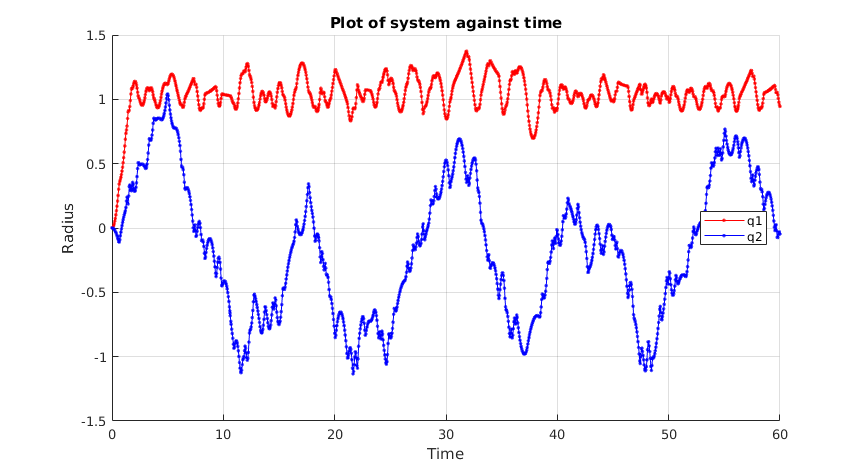
\includegraphics[scale=0.4]{quant2_2_2.png}
    \caption{Sampled controller test with quantization module for 4 degree and 4Nm levels}
    \label{fig:11}
\end{figure}  


\end{document}      % End of the document


%%%%%%%%%%%%%%%%%%%%%%%%%%%%%%%%%%%%%%%%%%%%%%%%%%%%%%%%%%%%%%%%%%%%%%%%%%%%%%%%%%%
% The bibliography
%%%%%%%%%%%%%%%%%%%%%%%%%%%%%%%%%%%%%%%%%%%%%%%%%%%%%%%%%%%%%%%%%%%%%%%%%%%%%%%%%%%
%\bibliography{Bibliography_template} %Read the bibliography from a separate file

\begin{thebibliography}{99}
\bibitem[Khalil(2002)]{Khalil:2002:Nonlinear-systems:vh}
Hassan~K Khalil.
\newblock \emph{Nonlinear systems}.
\newblock Prentice Hall, Upper Saddle river, 3. edition, 2002.
\newblock ISBN 0-13-067389-7.

\bibitem[Oetiker et~al.(2008)Oetiker, Partl, Hyna, and
  Schlegl]{Oetiker:2008:TheNotSoShortIntroductiontoLaTeXe}
Tobias Oetiker, Hubert Partl, Irene Hyna, and Elisabeth Schlegl.
\newblock \emph{The Not So Short Introduction to \LaTeXe}.
\newblock Oetiker, OETIKER+PARTNER AG, Aarweg 15, 4600 Olten, Switzerland,
  2008.
\newblock http://www.ctan.org/info/lshort/.

\bibitem[Sastry(1999)]{Sastry:1999:Nonlinear-systems:-analysis-stability-and-c%
ontrol:xr}
Shankar Sastry.
\newblock \emph{Nonlinear systems: analysis, stability, and control},
  volume~10.
\newblock Springer, New York, N.Y., 1999.
\newblock ISBN 0-387-98513-1.
\end{thebibliography}
